\section{Server}

\subsection{Architettura}

\begin{center}
	\begin{figure}[t]
		\makebox[\textwidth]{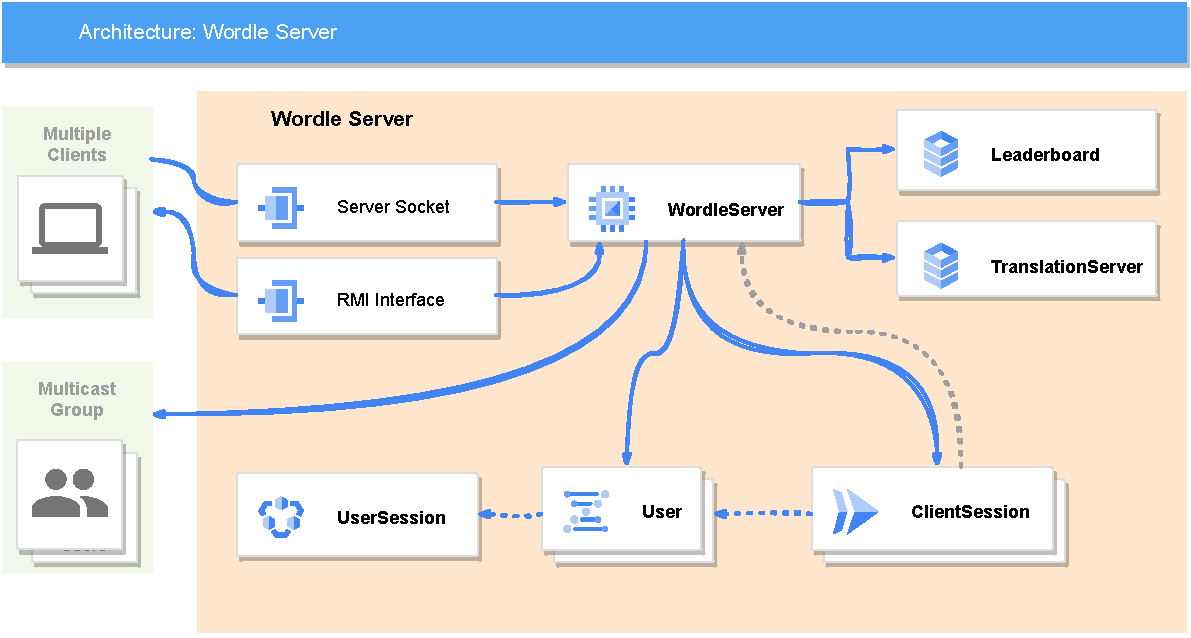
\includegraphics[width=0.7\paperwidth]{img/server_arch.pdf}}
		\caption{Rappresentazione dell'architettura del server. La linea tratteggiata blu indica che il riferimento e' opzionale (potrebbe non essere presente). Si noti che esiste una dipendenza circolare tra \textbf{WordleServer} e \textbf{ClientSession}, sarebbe stato possibile evitarla rendendo \textbf{ClientSession} una classe \texttt{private static} di \textbf{WordleServer} ma si avrebbe perso in chiarezza.}
		\label{fig:server_arch}
	\end{figure}
\end{center}

La struttura del server (raffigurata in figura \ref{fig:server_arch}) e' la seguente:
\bigskip

\dirtree{%
	.1 server/.
	.2 ServerMain \quad \begin{minipage}[t]{7cm}
		Entry point principale
	\end{minipage}.
    .2 WordleServer \quad \begin{minipage}[t]{7cm}
    	Core del server, istanza singleton
    \end{minipage}.
	.2 ClientSession \quad \begin{minipage}[t]{7cm}
		Gestisce la sessione di un client
	\end{minipage}.
	.2 Leaderboard \quad \begin{minipage}[t]{7cm}
		Struttura dati che contiene la classifica degli utenti
	\end{minipage}.
	.2 TranslationServer \quad \begin{minipage}[t]{7cm}
		Offre la traduzione in italiano delle secret word
	\end{minipage}.
	.2 User \quad \begin{minipage}[t]{7cm}
		Rappresenta un utente
	\end{minipage}.
	.2 UserSession \quad \begin{minipage}[t]{7cm}
		La sessione di un utente
	\end{minipage}.
	.2 logging/.
}
\bigskip

Il nucleo principale del server e' contenuto nella classe \textbf{WordleServer} che e' anche un oggetto singleton poiche' deve essere istanziato la prima volta da \textbf{ServerMain} e da quel momento in poi non deve essere mai piu' istanziato nuovamente, ne' terminato.

\newpage

\textbf{WordleServer} si occupa di:
\begin{itemize}
	\item Gestione della comunicazione con i client (tramite TCP, UDP e java RMI)
	\item Mantenimento delle informazioni persistenti relative agli utenti
	\item Registrazione e autenticazione degli utenti
	\item Generazione e validazione delle parole segrete
	\item Condivisione delle partite nel gruppo di multicast
	\item Traduzione della \emph{secret word}
	\item Notificare i client (\emph{subscribers}) quando avviene un cambiamento nelle prime posizioni in classifica
\end{itemize}

Tuttavia \textbf{WordleServer} non e' direttamente responsabile della logica della interazione con i client che invece e' affidata a \textbf{ClientSession}, il quale e' stato implementato come un semplice automa a stati finiti (raffigurato in Figura \ref{fig:clientsession_asf}), cosa che permette di verificarne facilmente la correttezza e quindi di garantire che il client si trovera' sempre in uno stato \emph{"safe"}.

\begin{center}
	\begin{figure}[t!]
		\makebox[\textwidth]{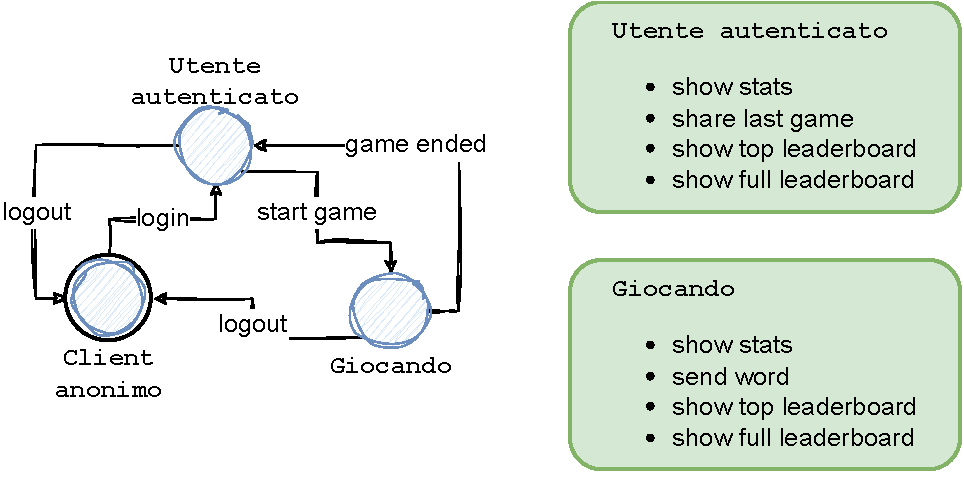
\includegraphics[width=0.6\paperwidth]{img/client_asf_v3.pdf}}
		\caption{A sinistra: descrizione dell'automa a stati finiti che gestisce l'interazione di un client col server (lo stato iniziale e' quello cerchiato). A destra: elenco dei comandi validi in ogni stato (questi comandi non cambiano lo stato corrente dell'automa).}
		\label{fig:clientsession_asf}
	\end{figure}
\end{center}

\subsection{TCP Socket}

Si e' scelto di gestire le connessioni TCP con dei socket I/O non bloccanti (\emph{Java NIO}) piuttosto che avere un pool di thread in cui ogni thread e' responsabile di un solo client.

Questa soluzione ci permette una migliore scalabilita' col numero di client, infatti un elevato numero di client che effettuano tuttavia poche operazioni causerebbe un enorme overhead se usassimo un thread ciascuno. In questo modo siamo limitati da un solo thread che gestisce le connessioni con dei dati pronti a essere letti o scritti.

In realta' la limitazione del thread singolo potrebbe essere rimossa qualora si sentisse il bisogno\footnote{Questa soluzione non e' stata adottata poiche' un tale livello di efficienza esula dagli obiettivi di questo progetto e l'implementazione risulta particolarmente insidiosa, tuttavia il resto del codice e' gia' stato predisposto per supportare una gestione parallela dei client} di migliorare ulteriormente l'efficienza sfruttando il parallelismo hardware (piu' core/CPU). In tal caso basterebbe delegare l'esecuzione di ciascun \textbf{ClientSession} a un pool di thread introducendo delle misure di sincronizzazione per evitare di elaborare due volte lo stesso messaggio.

\subsection{Leaderboard}

La classifica degli utenti e' gestita dalla classe \textbf{Leaderboard}. Internamente la classifica viene codificata con due strutture dati:
\begin{itemize}
	\item Un \textbf{BST} (\emph{Binary Search Tree}) in cui i nodi (che rappresentano gli utenti) sono ordinati per il \textbf{punteggio} dell'utente e sono etichettati con il relativo \textbf{username} (che ricordiamo essere unico)
	\item Una \textbf{hashmap} in cui la chiave e' lo \textbf{username} (se e solo se e' presente in classifica) e il valore associato e' un riferimento al nodo nel \textbf{BST} che identifica proprio quello username.
\end{itemize}
In questo modo sapere la posizione in classifica di un utente richiede $O(n)$ tempo mentre l'aggiunta, la rimozione e la modifica di una coppia (utente, punteggio) richiede $O(\log{n})$ tempo.

Vale la pena notare che usare un \textbf{Order Statistic Tree} al posto del \textbf{BST} comporterebbe un miglioramento della complessita' dell'operazione di \emph{rank}, ovvero sapere la posizione in classifica di un utente, che diventerebbe quindi $O(\log{n})$. Siccome l'implementazione di un \textbf{OST} non e' presente nella standard library di Java questa soluzione non e' stata utilizzata.

Praticamente l'implementazione non rispecchia totalmente la struttura definita sopra ma comporta alcune piccole modifiche che non cambiano la complessita' del problema:
\begin{itemize}
	\item Il \textbf{BST} e' stato implementato mediante una \textbf{TreeMap} in cui la chiave e' la coppia (ordinabile lessicograficamente) \emph{(punteggio, username)} mentre il valore non e' utilizzato.
	\item La \textbf{hashmap} e' stata implementata tramite una \textbf{HashMap} la cui chiave e' uno \emph{username} e il valore e' la coppia \emph{(punteggio, username)}.
\end{itemize}
Per mantenere sincronizzate entrambe le strutture dati e' necessario che tutti i metodi della classe \textbf{Leaderboard} siano mutualmente esclusivi, per fare cio' e' sufficiente dichiararli \textbf{synchronized}.

\subsection{Traduzione della secret word}

La traduzione della \emph{secret word} (gestita dalla classe \textbf{TranslationServer}) in italiano e' una procedura lenta che richiede di eseguire una richiesta HTTP e siccome si e' deciso di non utilizzare un thread pool per la gestione concorrente dei client l'intero server si blocca in attesa della risposta dal web server.

Per mitigare questo problema internamente viene usata una cache \textbf{LRU} (\emph{Least Recently Used}) che contiene la traduzione delle secret word. L'implementazione della cache \textbf{LRU} e' basata sulla \textbf{LinkedHashMap} offerta dalla standard library.

\subsection{Gestione della concorrenza}

Come precedentemente anticipato non ci sono molti thread che lavorano in parallelo. Tuttavia alcune componenti sono eseguite in un thread separato, in particolare la lista dei thread e':
\begin{itemize}
	\item Il main thread
	\item Flush scheduler: viene eseguito a intervalli regolari ed esegue la sincronizzazione con il file di salvataggio del server
	\item Thread per la generazione di una nuova secret word. Anche questo viene eseguito a intervalli regolari
	\item Shutdown hook: thread speciale che viene eseguito nel momento in cui il server inizia la fase di terminazione. Esegue un sync sul file di salvataggio.
	\item Share game: il thread si occupa di condividere una partita nel gruppo di multicast. Essendo questa di per se' una attivita' asincrona puo' essere eseguita tranquillamente da un thread separato
	\item Notifica ai subscribers. Anche questa attivita' puo' essere eseguita parallelamente siccome non viene generata direttamente da un client
	\item RMI threads: I metodi remoti disponibili possono generare molteplici thread. Il threadpool in questo caso e' gestito dalla \emph{JVM}
\end{itemize}

E' quindi necessario fare in modo che non si presentino situazioni di deadlock ne' altri problemi.

La maggior parte di questi thread opera su strutture dati dedicate o su tipi di dato primitivi (l'assegnamento in tal caso e' atomico), quindi le misure per la prevenzione di problemi dovuti all'accesso concorrente alle risorse sono molto semplici o addirittura assenti.

L'unica struttura dati che merita particolare attenzione e' la \textbf{map} \{\emph{username} : \emph{User}\} che associa a ogni \emph{username} il relativo oggetto di tipo \emph{User} che rappresenta l'utente. Tale struttura e' particolarmente delicata per i seguenti motivi:
\begin{enumerate}
	\item In fase di registrazione bisogna garantire l'atomicita' dell'operazione di creazione di un utente se gia' non esiste
	\item L'autenticazione, che consiste nel controllare se un utente esiste e in tal caso controllare se la password e' valida, deve essere atomica
	\item Durante la sincronizzazione dello stato del server in un file di salvataggio e' necessario operare su uno snapshot della lista di utenti \textbf{evitando} di scrivere informazioni corrotte o parziali
	\item Ogni istanza di \textbf{ClientSession} puo' operare sul relativo oggetto \textbf{User} ma non opera direttamente sulla \textbf{map} \{\emph{username} : \emph{User}\}
\end{enumerate}

Per risolvere questi problemi e mantenere comunque un alto livello di parallelismo si e' deciso di utilizzare una \textbf{ConcurrentHashMap} che, unita alle proprieta' che gli utenti non si possono eliminare e la password non si puo' cambiare, ci permette di risolvere i punti 1-2.

Per quanto riguarda il punto 4 si e' deciso di imporre un'altra proprieta':
\begin{quote}
	 In ogni istante successivo alla inizializzazione del server \underline{solo un} oggetto di tipo \textbf{ClientSession} puo' operare su un determinato oggetto \textbf{User}
\end{quote}

Infine il punto 3 si risolve imponendo che la classe \textbf{User} sia serializzabile previa cattura del lock tramite \textbf{synchronized}. Questo significa che le operazioni di modifica su \textbf{User} sono tutte atomiche e lasciano l'oggetto in uno stato corretto.

\subsection{Configurazione}

Nel file di configurazione \texttt{ServerMain.properties} si possono configurare i seguenti valori:
\begin{itemize}
	\item \texttt{multicast\_address}: l'indirizzo del gruppo di multicast
	\item \texttt{multicast\_port}: la porta da utilizzare quando si mandano messaggi nel gruppo di multicast
	\item \texttt{server\_port}: la porta da usare per il server socket
	\item \texttt{rmi\_port}: la porta da usare per i servizi RMI
	\item \texttt{verbose}: la verbosita' dei log (da 0 a 5)
	\item \texttt{secret\_word\_rate}: l'intervallo in secondi tra la generazione di una secret word e la successiva
	\item \texttt{words\_db}: file contenente la lista di parole	
\end{itemize}